\documentclass{article}

% content/resources/templates/preamble.tex
\usepackage[margin=0.6in]{geometry}
\author{Milav Dabgar}
\usepackage{amsmath,amssymb,amsthm}
\usepackage{booktabs}
\usepackage{multirow}
\usepackage{xcolor}
\usepackage{tcolorbox}
\tcbuselibrary{breakable,skins}
\usepackage[colorlinks=true,linkcolor=blue]{hyperref}
\usepackage{titlesec}
\usepackage{enumitem}
\usepackage{tikz}
\usepackage{pgfplots}
\usepackage{circuitikz}
\usepackage[version=4]{mhchem}
\usepackage{longtable}
\usepackage{array}
\usepackage{float}
\usepackage{caption}
\usepackage{listings}

\lstset{
  basicstyle=\small\ttfamily,
  breaklines=true,
  breakatwhitespace=false,
  postbreak=\mbox{\textcolor{red}{$\hookrightarrow$}\space},
  float=false,
  numbers=left,
  numberstyle=\tiny\color{gray},
  numbersep=10pt,
  xleftmargin=2em,
  keywordstyle=\color{blue},
  commentstyle=\color{green!60!black},
  stringstyle=\color{purple},
  backgroundcolor=\color{gray!5},
  showstringspaces=false,
  tabsize=2,
  captionpos=b,
  keepspaces=true,
  columns=flexible
}

\pgfplotsset{compat=1.18}
\usetikzlibrary{shapes,arrows,positioning,calc,patterns,decorations.pathmorphing,decorations.markings,arrows.meta}

% Color scheme
\definecolor{headcolor}{RGB}{0,102,204}
\definecolor{keycolor}{RGB}{220,20,60}
\definecolor{solutioncolor}{RGB}{34,139,34}
\definecolor{mnemoniccolor}{RGB}{148,0,211}
\definecolor{codecolor}{RGB}{0,0,100}

% Spacing
\setlength{\parskip}{3pt}
\setlist[itemize]{nosep}
\setlist[enumerate]{nosep}

% Title formatting
\titleformat{\section}{\Large\bfseries\color{headcolor}}{\thesection}{1em}{}
\titleformat{\subsection}{\large\bfseries\color{headcolor}}{\thesubsection}{1em}{}

% Pandoc tightlist compatibility
\providecommand{\tightlist}{%
  \setlength{\itemsep}{0pt}\setlength{\parskip}{0pt}}

% Pandoc longtable compatibility
\newcounter{none}
\def\thenone{}


% content/resources/templates/english-boxes.tex
% This file is currently empty - it exists to maintain consistency with the import structure.
% Add custom environments here if needed in the future.


% Custom commands for GTU solutions
% This file defines semantic commands for consistent formatting

% Question command with automatic formatting
\newcommand{\question}[2]{%
  \section*{Question #1}%
  \textbf{#2}%
}

% OR question variant
\newcommand{\questionor}[2]{%
  \section*{Question #1 OR}%
  \textbf{#2}%
}

% Proper table environment with caption
\newenvironment{answertable}[1]{%
  \begin{table}[htbp]
  \centering
  \caption{#1}
}{%
  \end{table}
}

% Proper figure environment for diagrams
\newenvironment{answerdiagram}[1]{%
  \begin{figure}[htbp]
  \centering
  \caption{#1}
}{%
  \end{figure}
}

% Semantic markup for key terms
\newcommand{\keyword}[1]{\textbf{#1}}
\newcommand{\code}[1]{\texttt{#1}}
\newcommand{\classname}[1]{\texttt{#1}}
\newcommand{\methodname}[1]{\texttt{#1}}

% Proper quotation marks
\newcommand{\mnemonic}[1]{``#1''}

\usetikzlibrary{mindmap,trees}

\title{Microprocessor and Microcontroller (4341101) - Summer 2025 Solution}
\date{May 13, 2025}

\begin{document}
\maketitle

\questionmarks{1}{a}{3}
\textbf{Define Microprocessor and draw its block diagram.}

\begin{solutionbox}
\textbf{Answer}:
A \textbf{microprocessor} is a programmable digital device that performs arithmetic and logical operations on data according to stored instructions.

\textbf{Block Diagram:}

\begin{center}
\begin{tikzpicture}[node distance=2.5cm, auto]
    \node [gtu block] (cpu) {CPU\\(Microprocessor)};
    \node [gtu block, left of=cpu, node distance=3.5cm] (input) {Input Device};
    \node [gtu block, right of=cpu, node distance=3.5cm] (output) {Output Device};
    \node [gtu block, below of=cpu, node distance=2.5cm] (memory) {Memory Unit};
    
    \draw [gtu arrow] (input) -- (cpu);
    \draw [gtu arrow] (cpu) -- (output);
    \draw [gtu arrow, <->] (cpu) -- (memory);
    
    % Internal CPU blocks visualization
    \node [draw, dashed, fit=(cpu), label=above:System Bus] {};
\end{tikzpicture}
\end{center}

\begin{itemize}
    \item \textbf{CPU}: Central Processing Unit performs all operations
    \item \textbf{Memory}: Stores programs and data
    \item \textbf{Control Unit}: Controls instruction execution sequence
\end{itemize}
\end{solutionbox}
\begin{mnemonicbox}
``My Computer Processes Instructions'' (Memory-CPU-Program-Instructions)
\end{mnemonicbox}

\questionmarks{1}{b}{4}
\textbf{Explain operand and opcode with proper instruction example.}

\begin{solutionbox}
\textbf{Answer}:
\textbf{Opcode} specifies the operation to be performed. \textbf{Operand} specifies the data on which operation is performed.

\textbf{Example Table:}

\begin{center}
\captionof{table}{Instruction Parts}
\begin{tabulary}{\linewidth}{|l|l|l|J|}
\hline
\textbf{Instruction} & \textbf{Opcode} & \textbf{Operand} & \textbf{Function} \\ \hline
\code{MOV A,B} & MOV & A,B & Move B to A \\ \hline
\code{ADD A,\#05H} & ADD & A,\#05H & Add 05H to A \\ \hline
\end{tabulary}
\end{center}

\begin{itemize}
    \item \textbf{Opcode}: Operation code (MOV, ADD, SUB)
    \item \textbf{Operand}: Data or address (A, B, \#05H)
    \item \textbf{Format}: Opcode + Operand = Complete Instruction
\end{itemize}
\end{solutionbox}
\begin{mnemonicbox}
``Operation On Data'' (Opcode-Operand-Data)
\end{mnemonicbox}

\questionmarks{1}{c}{7}
\textbf{Compare Microprocessor and Microcontroller.}

\begin{solutionbox}
\textbf{Answer}:

\begin{center}
\captionof{table}{Comparison}
\begin{tabulary}{\linewidth}{|l|J|J|}
\hline
\textbf{Parameter} & \textbf{Microprocessor} & \textbf{Microcontroller} \\ \hline
\textbf{Definition} & CPU only & CPU + Memory + I/O \\ \hline
\textbf{Memory} & External RAM/ROM & Internal RAM/ROM \\ \hline
\textbf{I/O Ports} & External interface & Built-in ports \\ \hline
\textbf{Cost} & Higher system cost & Lower system cost \\ \hline
\textbf{Power} & Higher consumption & Lower consumption \\ \hline
\textbf{Speed} & Faster processing & Moderate speed \\ \hline
\textbf{Applications} & Computers, laptops & Washing machine, microwave \\ \hline
\end{tabulary}
\end{center}

\begin{itemize}
    \item \textbf{Microprocessor}: General purpose computing
    \item \textbf{Microcontroller}: Specific embedded applications
    \item \textbf{Integration}: Microcontroller has everything on single chip
\end{itemize}
\end{solutionbox}
\begin{mnemonicbox}
``Micro Means More Integration'' (Microcontroller-Memory-More-Integration)
\end{mnemonicbox}

\orquestionmarks{1}{c}{7}
\textbf{Compare RISC and CISC.}

\begin{solutionbox}
\textbf{Answer}:

\begin{center}
\captionof{table}{RISC vs CISC}
\begin{tabulary}{\linewidth}{|l|J|J|}
\hline
\textbf{Parameter} & \textbf{RISC} & \textbf{CISC} \\ \hline
\textbf{Instructions} & Simple, few & Complex, many \\ \hline
\textbf{Instruction Size} & Fixed length & Variable length \\ \hline
\textbf{Execution Time} & Single cycle & Multiple cycles \\ \hline
\textbf{Memory Access} & Load/Store only & Any instruction \\ \hline
\textbf{Registers} & More registers & Fewer registers \\ \hline
\textbf{Pipeline} & Efficient pipelining & Complex pipelining \\ \hline
\textbf{Examples} & ARM, MIPS & x86, 8085 \\ \hline
\end{tabulary}
\end{center}

\begin{itemize}
    \item \textbf{RISC}: Reduced Instruction Set Computer
    \item \textbf{CISC}: Complex Instruction Set Computer
    \item \textbf{Performance}: RISC faster, CISC more flexible
\end{itemize}
\end{solutionbox}
\begin{mnemonicbox}
``Reduced Instructions Speed Computing'' (RISC-Instructions-Speed-Computing)
\end{mnemonicbox}

\questionmarks{2}{a}{3}
\textbf{Explain Bus Organization of 8085 microprocessor.}

\begin{solutionbox}
\textbf{Answer}:
8085 has \textbf{three types} of buses for communication with external devices.

\begin{center}
\captionof{table}{Bus Organization}
\begin{tabulary}{\linewidth}{|l|l|J|}
\hline
\textbf{Bus Type} & \textbf{Lines} & \textbf{Function} \\ \hline
\textbf{Address Bus} & 16 lines (A0-A15) & Memory addressing \\ \hline
\textbf{Data Bus} & 8 lines (D0-D7) & Data transfer \\ \hline
\textbf{Control Bus} & Multiple lines & Control signals \\ \hline
\end{tabulary}
\end{center}

\begin{itemize}
    \item \textbf{Address Bus}: Unidirectional, 64KB memory addressing
    \item \textbf{Data Bus}: Bidirectional, 8-bit data transfer
    \item \textbf{Control Bus}: Read, Write, IO/M signals
\end{itemize}
\end{solutionbox}
\begin{mnemonicbox}
``Address Data Control'' (ADC)
\end{mnemonicbox}

\questionmarks{2}{b}{4}
\textbf{Explain function of ALE signal with diagram.}

\begin{solutionbox}
\textbf{Answer}:
\textbf{ALE (Address Latch Enable)} separates address and data on multiplexed bus.

\textbf{ALE Timing Diagram:}

\begin{center}
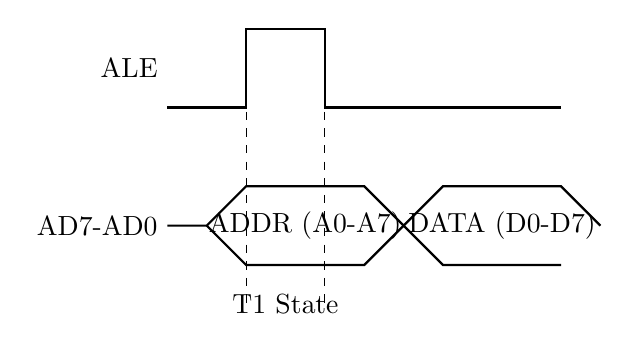
\begin{tikzpicture}[scale=1, transform shape]
    % ALE Waveform
    \draw [thick] (0, 0) -- (1, 0) -- (1, 1) -- (2, 1) -- (2, 0) -- (5, 0);
    \node [left] at (0, 0.5) {ALE};
    
    % AD Bus
    \draw [thick] (0, -1.5) -- (0.5, -1.5) -- (1, -1) -- (2.5, -1) -- (3, -1.5) -- (3.5, -1) -- (5, -1) -- (5.5, -1.5);
    \draw [thick] (0.5, -1.5) -- (1, -2) -- (2.5, -2) -- (3, -1.5) -- (3.5, -2) -- (5, -2);
    
    \node [left] at (0, -1.5) {AD7-AD0};
    \node at (1.75, -1.5) {ADDR (A0-A7)};
    \node at (4.25, -1.5) {DATA (D0-D7)};
    
    % Dashed lines
    \draw [dashed] (1, 1) -- (1, -2.5);
    \draw [dashed] (2, 1) -- (2, -2.5);
    \node at (1.5, -2.5) {T1 State};
\end{tikzpicture}
\end{center}

\begin{itemize}
    \item \textbf{High ALE}: Address is available on AD0-AD7
    \item \textbf{Low ALE}: Data is available on AD0-AD7
    \item \textbf{Function}: Latches lower address byte
    \item \textbf{Frequency}: ALE = Clock frequency $\div$ 2
\end{itemize}
\end{solutionbox}
\begin{mnemonicbox}
``Address Latch Enable'' (ALE)
\end{mnemonicbox}

\questionmarks{2}{c}{7}
\textbf{Describe architecture of 8085 microprocessor with the help of neat diagram.}

\begin{solutionbox}
\textbf{Answer}:

\textbf{Diagram:}

\begin{center}
\begin{tikzpicture}[node distance=2.5cm, auto, scale=0.8, transform shape]
    % Registers
    \node [gtu block, minimum width=2cm] (acc) {Accumulator\\(8)};
    \node [gtu block, right of=acc, node distance=3cm, minimum width=2cm] (tr) {Temp Reg\\(8)};
    \node [gtu block, below of=acc, node distance=2cm, minimum width=2cm] (fr) {Flag Reg\\(5)};
    \node [gtu block, right of=fr, node distance=3cm] (alu) {ALU\\(8)};
    
    \node [gtu block, right of=tr, node distance=4cm, minimum width=3cm] (regs) {B(8) | C(8)\\D(8) | E(8)\\H(8) | L(8)};
    \node [gtu block, below of=regs, node distance=2.5cm, minimum width=3cm] (sp) {Stack Pointer (16)};
    \node [gtu block, below of=sp, node distance=1.5cm, minimum width=3cm] (pc) {Prog Counter (16)};
    
    % Buses
    \node [gtu block, below of=fr, node distance=4cm, minimum width=8cm] (bus) {Internal Data Bus (8)};
    
    % Control
    \node [gtu block, left of=bus, node distance=6cm] (control) {Timing \&\\Control Unit};
    \node [gtu block, above of=control] (ir) {Instruction\\Register};
    \node [gtu block, right of=ir] (id) {Decoder};
    
    % Connections
    \draw [gtu arrow, <->] (acc) -- (bus.160);
    \draw [gtu arrow, <->] (regs) -- (bus.20);
    \draw [gtu arrow] (tr) -- (alu);
    \draw [gtu arrow] (acc) -- (alu);
    \draw [gtu arrow] (alu) -- (fr);
    \draw [gtu arrow] (alu) -- (bus);
    
    \draw [gtu arrow] (bus) -| (ir);
    \draw [gtu arrow] (ir) -- (id);
    \draw [gtu arrow] (id) -- (control);
    
    % External
    \node [below of=bus, node distance=1.5cm] (buffers) {Address/Data Buffers};
    \draw [gtu arrow, <->] (bus) -- (buffers);

\end{tikzpicture}
\end{center}

\textbf{Key Components:}
\begin{itemize}
    \item \textbf{ALU}: Performs arithmetic and logical operations
    \item \textbf{Registers}: Store temporary data (A, B, C, D, E, H, L)
    \item \textbf{Program Counter}: Points to next instruction
    \item \textbf{Stack Pointer}: Points to stack top
    \item \textbf{Control Unit}: Generates control signals
\end{itemize}
\end{solutionbox}
\begin{mnemonicbox}
``All Registers Program Stack Control'' (A-R-P-S-C)
\end{mnemonicbox}

\orquestionmarks{2}{a}{3}
\textbf{Draw Flag Register of 8085 microprocessor \& explain it.}

\begin{solutionbox}
\textbf{Answer}:

\textbf{Flag Register Format:}

\begin{center}
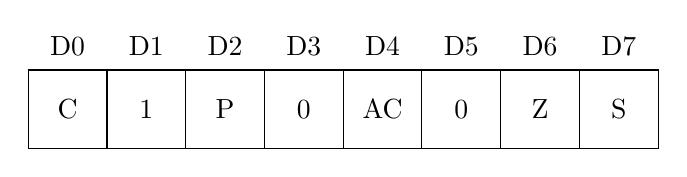
\begin{tikzpicture}
    \foreach \x/\label in {0/C, 1/1, 2/P, 3/0, 4/AC, 5/0, 6/Z, 7/S} {
        \draw (\x,0) rectangle (\x+1,1);
        \node at (\x+0.5, 0.5) {\label};
        \node at (\x+0.5, 1.3) {D\x};
    }
\end{tikzpicture}
\end{center}

\textbf{Flag Functions:}
\begin{itemize}
    \item \textbf{S (Sign)}: Set if result is negative
    \item \textbf{Z (Zero)}: Set if result is zero
    \item \textbf{AC (Auxiliary Carry)}: Set for BCD operations (carry from D3 to D4)
    \item \textbf{P (Parity)}: Set for even parity
    \item \textbf{C (Carry)}: Set when carry/borrow occurs
\end{itemize}
\end{solutionbox}
\begin{mnemonicbox}
``Some Zero Auxiliary Parity Carry'' (SZAPC)
\end{mnemonicbox}

\orquestionmarks{2}{b}{4}
\textbf{Explain De-multiplexing of Address and Data buses for 8085 Microprocessor.}

\begin{solutionbox}
\textbf{Answer}:
\textbf{De-multiplexing} separates address and data signals from AD0-AD7 lines.

\textbf{De-multiplexing Circuit:}

\begin{center}
\begin{tikzpicture}[node distance=3cm, auto]
    \node (8085) [draw, minimum height=3cm] {8085};
    \node (latch) [gtu block, right of=8085, node distance=4cm] {Latch\\(74LS373)};
    
    \draw [thick] (8085.east) -- (latch.west) node[midway, above] {AD0-AD7};
    \draw [->, thick] (latch.east) -- ++(2,0) node[right] {A0-A7 (Address)};
    
    \draw [->, thick] ($(8085.east)+(2,0)$) -- ++(0, -1.5) -- ++(2,0) node[right] {D0-D7 (Data)};
    
    \draw [->, dashed] ($(8085.east)+(0,1)$) node[left] {ALE} -| (latch.north);
\end{tikzpicture}
\end{center}

\begin{itemize}
    \item \textbf{ALE High}: Address latched in external latch (A0-A7)
    \item \textbf{ALE Low}: Data flows through buffer (D0-D7)
    \item \textbf{74LS373}: Common latch IC used
    \item \textbf{Benefit}: Separate address and data buses
\end{itemize}
\end{solutionbox}
\begin{mnemonicbox}
``Address Latch External Demultiplex'' (ALED)
\end{mnemonicbox}

\orquestionmarks{2}{c}{7}
\textbf{Describe Pin diagram of 8085 microprocessor with the help of neat diagram.}

\begin{solutionbox}
\textbf{Answer}:

\begin{center}
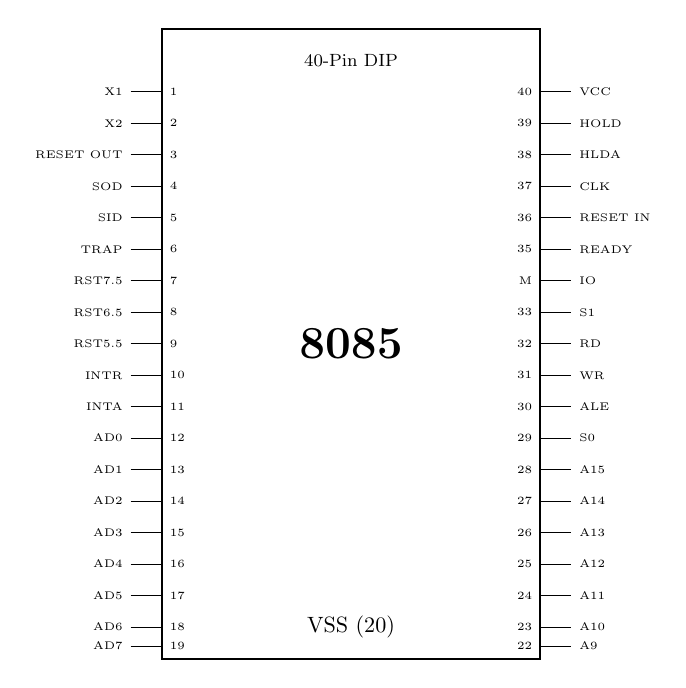
\begin{tikzpicture}[scale=0.8, transform shape]
    \draw [thick] (0,0) rectangle (6,10);
    \node at (3,5) {\huge \textbf{8085}};
    \node at (3,9.5) {\footnotesize 40-Pin DIP};
    
    % Left Pins
    \foreach \y/\label/\pin in {9/X1/1, 8.5/X2/2, 8/RESET OUT/3, 7.5/SOD/4, 7/SID/5, 6.5/TRAP/6, 6/RST7.5/7, 5.5/RST6.5/8, 5/RST5.5/9, 4.5/INTR/10, 4/INTA/11, 3.5/AD0/12, 3/AD1/13, 2.5/AD2/14, 2/AD3/15, 1.5/AD4/16, 1/AD5/17, 0.5/AD6/18} {
        \draw (-0.5, \y) -- (0, \y);
        \node [left] at (-0.5, \y) {\tiny \label};
        \node [right] at (0, \y) {\tiny \pin};
    }
    
    % Right Pins
    \foreach \y/\label/\pin in {9/VCC/40, 8.5/HOLD/39, 8/HLDA/38, 7.5/CLK/37, 7/RESET IN/36, 6.5/READY/35, 6/IO/M/34, 5.5/S1/33, 5/RD/32, 4.5/WR/31, 4/ALE/30, 3.5/S0/29, 3/A15/28, 2.5/A14/27, 2/A13/26, 1.5/A12/25, 1/A11/24, 0.5/A10/23} {
        \draw (6, \y) -- (6.5, \y);
        \node [right] at (6.5, \y) {\tiny \label};
        \node [left] at (6, \y) {\tiny \pin};
    }
    
    % Bottom pins
    \draw (-0.5, 0.2) -- (0, 0.2); \node [left] at (-0.5, 0.2) {\tiny AD7}; \node [right] at (0, 0.2) {\tiny 19};
    \draw (6, 0.2) -- (6.5, 0.2); \node [right] at (6.5, 0.2) {\tiny A9}; \node [left] at (6, 0.2) {\tiny 22};
    
    \node at (3, 0.5) {VSS (20)};
\end{tikzpicture}
\end{center}

\textbf{Pin Categories:}
\begin{itemize}
    \item \textbf{Power}: VCC (+5V), VSS (GND)
    \item \textbf{Clock}: X1, X2 (Crystal), CLK OUT
    \item \textbf{Address/Data}: AD0-AD7 (Multiplexed), A8-A15 (High Address)
    \item \textbf{Control}: ALE, RD, WR, IO/M, S0, S1
    \item \textbf{Interrupt}: INTR, INTA, RST7.5, RST6.5, RST5.5, TRAP
\end{itemize}
\end{solutionbox}
\begin{mnemonicbox}
``Power Clock Address Control Interrupt'' (PCACI)
\end{mnemonicbox}

\questionmarks{3}{a}{3}
\textbf{Write a function of DPTR and PC.}

\begin{solutionbox}
\textbf{Answer}:

\begin{center}
\captionof{table}{Functions}
\begin{tabulary}{\linewidth}{|l|J|l|}
\hline
\textbf{Register} & \textbf{Function} & \textbf{Size} \\ \hline
\textbf{DPTR} & Data Pointer & 16-bit \\ \hline
\textbf{PC} & Program Counter & 16-bit \\ \hline
\end{tabulary}
\end{center}

\begin{itemize}
    \item \textbf{DPTR Functions}:
    \begin{itemize}
        \item Access external data memory (RAM/ROM)
        \item Holds 16-bit address for \code{MOVX A,@DPTR} or \code{MOVC A,@A+DPTR}
    \end{itemize}
    \item \textbf{PC Functions}:
    \begin{itemize}
        \item Points to the address of the \textbf{next instruction} to be executed
        \item Auto-increments after each instruction fetch
    \end{itemize}
\end{itemize}
\end{solutionbox}
\begin{mnemonicbox}
``Data Program Counter'' (DPC)
\end{mnemonicbox}

\questionmarks{3}{b}{4}
\textbf{Draw PCON SFR of 8051 and Explain function of each bit.}

\begin{solutionbox}
\textbf{Answer}:

\textbf{PCON Register (87H):}

\begin{center}
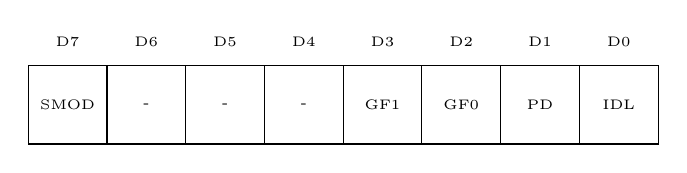
\begin{tikzpicture}
    \foreach \x/\label/\bit in {0/SMOD/D7, 1/-/D6, 2/-/D5, 3/-/D4, 4/GF1/D3, 5/GF0/D2, 6/PD/D1, 7/IDL/D0} {
        \draw (\x,0) rectangle (\x+1,1);
        \node at (\x+0.5, 0.5) {\tiny \label};
        \node at (\x+0.5, 1.3) {\tiny \bit};
    }
\end{tikzpicture}
\end{center}

\textbf{Bit Functions:}
\begin{itemize}
    \item \textbf{SMOD (D7)}: Serial port baud rate doubler (if set, baud rate is doubled in Mode 1, 2, 3)
    \item \textbf{GF1, GF0 (D3, D2)}: General purpose user flags
    \item \textbf{PD (D1)}: Power Down mode (Oscillator stops, minimal power)
    \item \textbf{IDL (D0)}: Idle mode (Clock to CPU stops, peripherals active)
\end{itemize}
\end{solutionbox}
\begin{mnemonicbox}
``Serial General Power Idle'' (SGPI)
\end{mnemonicbox}

\questionmarks{3}{c}{7}
\textbf{Explain architecture of 8051 microcontroller with the help of neat diagram.}

\begin{solutionbox}
\textbf{Answer}:

\textbf{Diagram:}

\begin{center}
\begin{tikzpicture}[node distance=2.5cm, auto, scale=0.8, transform shape]
    \node [gtu block] (cpu) {CPU};
    \node [gtu block, right of=cpu, node distance=3cm] (osc) {Oscillator};
    \node [gtu block, below of=cpu] (int) {Interrupt\\Control};
    \node [gtu block, right of=int, node distance=3cm] (bus) {Bus Control};
    
    \node [gtu block, left of=cpu, node distance=3.5cm] (rom) {4KB ROM};
    \node [gtu block, below of=rom] (ram) {128B RAM};
    
    \node [gtu block, right of=osc, node distance=3cm] (timers) {Timer 0\\Timer 1};
    \node [gtu block, below of=timers] (serial) {Serial Port\\(UART)};
    
    \node [gtu block, below of=int, minimum width=8cm] (ports) {I/O Ports (P0, P1, P2, P3)};
    
    \draw [gtu arrow, <->] (cpu) -- (rom);
    \draw [gtu arrow, <->] (cpu) -- (ram);
    \draw [gtu arrow] (osc) -- (cpu);
    \draw [gtu arrow] (int) -- (cpu);
    \draw [gtu arrow, <->] (cpu) -- (bus);
    \draw [gtu arrow, <->] (bus) -- (ports);
    \draw [gtu arrow, <->] (timers) -- (bus);
    \draw [gtu arrow, <->] (serial) -- (bus);
    
    \node [draw, dashed, fit=(cpu) (ports) (ram) (serial)] {};
\end{tikzpicture}
\end{center}

\textbf{Major Blocks:}
\begin{itemize}
    \item \textbf{CPU}: 8-bit processor with ALU and Accumulator
    \item \textbf{Memory}: 4KB Internal ROM (Code), 128B Internal RAM (Data)
    \item \textbf{Timers}: Two 16-bit timers/counters (T0, T1)
    \item \textbf{Serial Port}: Full duplex UART (TXD, RXD)
    \item \textbf{I/O Ports}: Four 8-bit bidirectional ports (P0-P3)
    \item \textbf{Interrupts}: 5 interrupt sources (External 0/1, Timer 0/1, Serial)
\end{itemize}
\end{solutionbox}
\begin{mnemonicbox}
``CPU Memory Timer Serial IO Interrupt'' (CMTSII)
\end{mnemonicbox}

\orquestionmarks{3}{a}{3}
\textbf{List common features of 8051 microcontroller.}

\begin{solutionbox}
\textbf{Answer}:
\textbf{Common Features:}
\begin{itemize}
    \item \textbf{CPU}: 8-bit microcontroller
    \item \textbf{Memory}: 4KB On-chip Program Memory (ROM), 128 Bytes On-chip Data Memory (RAM)
    \item \textbf{I/O Ports}: 32 I/O lines arranged as four 8-bit ports (P0-P3)
    \item \textbf{Timers}: Two 16-bit timers/counters (T0 and T1)
    \item \textbf{Serial Port}: One Full duplex UART serial channel
    \item \textbf{Interrupts}: 5 interrupt sources (2 External, 2 Timers, 1 Serial)
    \item \textbf{Clock}: On-chip oscillator (typically 12MHz)
\end{itemize}
\end{solutionbox}
\begin{mnemonicbox}
``CPU Memory IO Timer Serial Interrupt Clock'' (CMITSIC)
\end{mnemonicbox}

\orquestionmarks{3}{b}{4}
\textbf{Draw IP SFR of 8051 and Explain function of each bit.}

\begin{solutionbox}
\textbf{Answer}:

\textbf{IP Register (B8H) - Interrupt Priority:}

\begin{center}
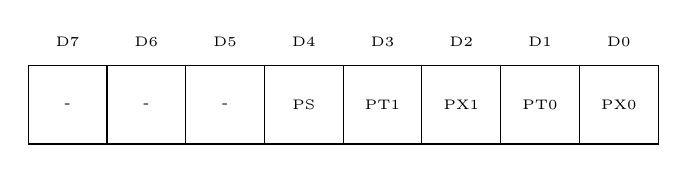
\begin{tikzpicture}
    \foreach \x/\label/\bit in {0/-/D7, 1/-/D6, 2/-/D5, 3/PS/D4, 4/PT1/D3, 5/PX1/D2, 6/PT0/D1, 7/PX0/D0} {
        \draw (\x,0) rectangle (\x+1,1);
        \node at (\x+0.5, 0.5) {\tiny \label};
        \node at (\x+0.5, 1.3) {\tiny \bit};
    }
\end{tikzpicture}
\end{center}

\textbf{Bit Functions:}
\begin{itemize}
    \item \textbf{PS}: Serial Port Interrupt Priority
    \item \textbf{PT1}: Timer 1 Interrupt Priority
    \item \textbf{PX1}: External Interrupt 1 Priority
    \item \textbf{PT0}: Timer 0 Interrupt Priority
    \item \textbf{PX0}: External Interrupt 0 Priority
\end{itemize}
\textbf{Priority Levels:} 1 = High Priority, 0 = Low Priority
\end{solutionbox}
\begin{mnemonicbox}
``Priority Serial Timer External'' (PSTE)
\end{mnemonicbox}

\orquestionmarks{3}{c}{7}
\textbf{With the help of neat diagram explain Pin diagram of 8051 microcontroller.}

\begin{solutionbox}
\textbf{Answer}:

\begin{center}
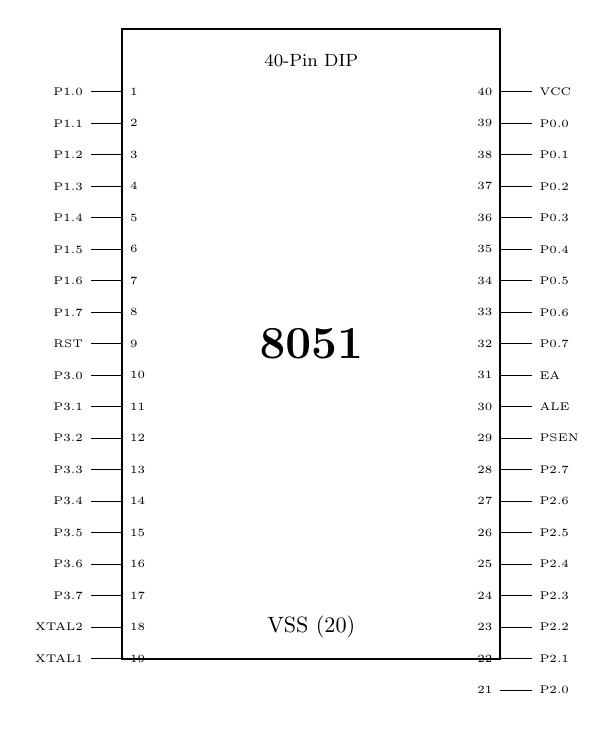
\begin{tikzpicture}[scale=0.8, transform shape]
    \draw [thick] (0,0) rectangle (6,10);
    \node at (3,5) {\huge \textbf{8051}};
    \node at (3,9.5) {\footnotesize 40-Pin DIP};
    
    % Left Pins (1-20)
    \foreach \y/\label/\pin in {9/P1.0/1, 8.5/P1.1/2, 8/P1.2/3, 7.5/P1.3/4, 7/P1.4/5, 6.5/P1.5/6, 6/P1.6/7, 5.5/P1.7/8, 5/RST/9, 4.5/P3.0/10, 4/P3.1/11, 3.5/P3.2/12, 3/P3.3/13, 2.5/P3.4/14, 2/P3.5/15, 1.5/P3.6/16, 1/P3.7/17, 0.5/XTAL2/18} {
        \draw (-0.5, \y) -- (0, \y);
        \node [left] at (-0.5, \y) {\tiny \label};
        \node [right] at (0, \y) {\tiny \pin};
    }
    \draw (-0.5, 0) -- (0, 0); \node [left] at (-0.5, 0) {\tiny XTAL1}; \node [right] at (0, 0) {\tiny 19};
    \node at (3, 0.5) {VSS (20)};
    
    % Right Pins (21-40)
    \foreach \y/\label/\pin in {9/VCC/40, 8.5/P0.0/39, 8/P0.1/38, 7.5/P0.2/37, 7/P0.3/36, 6.5/P0.4/35, 6/P0.5/34, 5.5/P0.6/33, 5/P0.7/32, 4.5/EA/31, 4/ALE/30, 3.5/PSEN/29, 3/P2.7/28, 2.5/P2.6/27, 2/P2.5/26, 1.5/P2.4/25, 1/P2.3/24, 0.5/P2.2/23} {
        \draw (6, \y) -- (6.5, \y);
        \node [right] at (6.5, \y) {\tiny \label};
        \node [left] at (6, \y) {\tiny \pin};
    }
    \draw (6, 0) -- (6.5, 0); \node [right] at (6.5, 0) {\tiny P2.1}; \node [left] at (6, 0) {\tiny 22};
    \draw (6, -0.5) -- (6.5, -0.5); \node [right] at (6.5, -0.5) {\tiny P2.0}; \node [left] at (6, -0.5) {\tiny 21};
\end{tikzpicture}
\end{center}

\textbf{Pin Groups:}
\begin{itemize}
    \item \textbf{Power}: VCC (40), VSS (20)
    \item \textbf{Clock}: XTAL1, XTAL2 (Oscillator)
    \item \textbf{Reset}: RST (High active reset)
    \item \textbf{Ports}:
    \begin{itemize}
        \item P0 (32-39): Address/Data bus
        \item P1 (1-8): I/O only
        \item P2 (21-28): High Address
        \item P3 (10-17): Special functions (Serial, Interrupts, Timers)
    \end{itemize}
    \item \textbf{Control}: ALE, PSEN, EA
\end{itemize}
\end{solutionbox}
\begin{mnemonicbox}
``Power Clock Reset Ports Control'' (PCRPC)
\end{mnemonicbox}

\questionmarks{4}{a}{3}
\textbf{Explain arithmetic instructions with example.}

\begin{solutionbox}
\textbf{Answer}:

\textbf{Arithmetic Instructions:}

\begin{center}
\captionof{table}{Arithmetic Instructions}
\begin{tabulary}{\linewidth}{|l|l|J|}
\hline
\textbf{Instruction} & \textbf{Function} & \textbf{Example} \\ \hline
\textbf{ADD} & Addition & \code{ADD A,\#10H} \\ \hline
\textbf{SUBB} & Subtraction & \code{SUBB A,R0} \\ \hline
\textbf{MUL} & Multiplication & \code{MUL AB} \\ \hline
\textbf{DIV} & Division & \code{DIV AB} \\ \hline
\textbf{INC} & Increment & \code{INC A} \\ \hline
\textbf{DEC} & Decrement & \code{DEC R1} \\ \hline
\end{tabulary}
\end{center}

\begin{itemize}
    \item \code{ADD A,\#10H}: Add 10H to accumulator
    \item \textbf{Flags}: Affected by arithmetic operations (C, AC, OV, P)
\end{itemize}
\end{solutionbox}
\begin{mnemonicbox}
``Add Subtract Multiply Divide Increment Decrement'' (ASMIDI)
\end{mnemonicbox}

\questionmarks{4}{b}{4}
\textbf{Write an 8051 Assembly Language Program to Find 2's complement of a value stored at memory location 65H. Put the result on same location.}

\begin{solutionbox}
\textbf{Answer}:

\begin{lstlisting}[language={[x86masm]Assembler}]
ORG 0000H           ; Program start address
MOV A,65H           ; Load value from location 65H
CPL A               ; Complement the value (1's complement)
ADD A,#01H          ; Add 1 to get 2's complement
MOV 65H,A           ; Store result back to 65H
SJMP $              ; Stop program
END
\end{lstlisting}

\textbf{Program Steps:}
\begin{itemize}
    \item \textbf{Load}: Get value from memory location 65H
    \item \textbf{Complement}: Generate 1's complement using CPL
    \item \textbf{Add 1}: Convert to 2's complement
    \item \textbf{Store}: Put result back to same location
\end{itemize}
\end{solutionbox}
\begin{mnemonicbox}
``Load Complement Add Store'' (LCAS)
\end{mnemonicbox}

\questionmarks{4}{c}{7}
\textbf{List Addressing Modes of 8051 Microcontroller and explain them with example.}

\begin{solutionbox}
\textbf{Answer}:

\begin{center}
\captionof{table}{Addressing Modes}
\begin{tabulary}{\linewidth}{|l|J|l|J|}
\hline
\textbf{Mode} & \textbf{Description} & \textbf{Example} & \textbf{Usage} \\ \hline
\textbf{Immediate} & Data directly in instruction & \code{MOV A,\#25H} & Constant data \\ \hline
\textbf{Register} & Data in register & \code{MOV A,R0} & Fast access \\ \hline
\textbf{Direct} & Memory address specified & \code{MOV A,30H} & RAM access \\ \hline
\textbf{Indirect} & Address stored in register & \code{MOV A,@R0} & Pointer/Array access \\ \hline
\textbf{Indexed} & Base address + offset & \code{MOVC A,@A+DPTR} & Table lookup \\ \hline
\textbf{Relative} & Jump amount relative to PC & \code{SJMP LOOP} & Branching \\ \hline
\textbf{Bit} & Operations on single bit & \code{SETB P1.0} & Bit manipulation \\ \hline
\end{tabulary}
\end{center}

\textbf{Examples:}
\begin{itemize}
    \item \code{MOV A,\#25H}: Load immediate value 25H
    \item \code{MOV A,@R0}: Load data from address held in R0
    \item \code{SJMP LOOP}: Jump to label LOOP (relative to current PC)
\end{itemize}
\end{solutionbox}
\begin{mnemonicbox}
``Immediate Register Direct Indirect Indexed Relative Bit'' (IRDIIRB)
\end{mnemonicbox}

\orquestionmarks{4}{a}{3}
\textbf{Explain logical instruction with example.}

\begin{solutionbox}
\textbf{Answer}:

\textbf{Logical Instructions:}

\begin{center}
\captionof{table}{Logical Instructions}
\begin{tabulary}{\linewidth}{|l|l|J|}
\hline
\textbf{Instruction} & \textbf{Function} & \textbf{Example} \\ \hline
\textbf{ANL} & AND operation & \code{ANL A,\#0FH} \\ \hline
\textbf{ORL} & OR operation & \code{ORL A,R1} \\ \hline
\textbf{XRL} & XOR operation & \code{XRL A,\#55H} \\ \hline
\textbf{CPL} & Complement & \code{CPL A} \\ \hline
\textbf{RL} & Rotate Left & \code{RL A} \\ \hline
\textbf{RR} & Rotate Right & \code{RR A} \\ \hline
\end{tabulary}
\end{center}

\begin{itemize}
    \item \code{ANL A,\#0FH}: AND accumulator with 0FH (Masking example)
    \item \textbf{Applications}: Bit masking, data manipulation, flag testing
\end{itemize}
\end{solutionbox}
\begin{mnemonicbox}
``AND OR XOR Complement Rotate'' (AOXCR)
\end{mnemonicbox}

\orquestionmarks{4}{b}{4}
\textbf{Write an 8051 Assembly Language Program to Multiply the number in register R3 by the number in register R0 and put the result in internal RAM location 10h(MSB) and 11h(LSB).}

\begin{solutionbox}
\textbf{Answer}:

\begin{lstlisting}[language={[x86masm]Assembler}]
ORG 0000H           ; Program start address
MOV A,R3            ; Move multiplicand (R3) to Accumulator
MOV B,R0            ; Move multiplier (R0) to B register
MUL AB              ; Multiply A by B (Product: B=High, A=Low)
MOV 10H,B           ; Store MSB (B) to location 10H
MOV 11H,A           ; Store LSB (A) to location 11H  
SJMP $              ; Stop program
END
\end{lstlisting}

\textbf{Program Flow:}
\begin{itemize}
    \item \textbf{Load}: Move multiplicand and multiplier to specific registers (A and B)
    \item \textbf{Multiply}: Execute \code{MUL AB} to perform 8-bit $\times$ 8-bit multiplication
    \item \textbf{Result}: 16-bit product is stored in B (High Byte) and A (Low Byte)
    \item \textbf{Store}: Save MSB and LSB to specified RAM locations
\end{itemize}
\end{solutionbox}
\begin{mnemonicbox}
``Load Multiply Store Result'' (LMSR)
\end{mnemonicbox}

\orquestionmarks{4}{c}{7}
\textbf{Explain data transfer instruction with example.}

\begin{solutionbox}
\textbf{Answer}:

\textbf{Data Transfer Instructions:}

\begin{center}
\captionof{table}{Data Transfer Instructions}
\begin{tabulary}{\linewidth}{|l|l|J|l|}
\hline
\textbf{Category} & \textbf{Instruction} & \textbf{Example} & \textbf{Function} \\ \hline
\textbf{Register} & MOV & \code{MOV A,R0} & Register to register \\ \hline
\textbf{Immediate} & MOV & \code{MOV A,\#25H} & Immediate to register \\ \hline
\textbf{Direct} & MOV & \code{MOV A,30H} & Memory to register \\ \hline
\textbf{Indirect} & MOV & \code{MOV A,@R0} & Indirect addressing \\ \hline
\textbf{External} & MOVX & \code{MOVX A,@DPTR} & External data memory \\ \hline
\textbf{Code} & MOVC & \code{MOVC A,@A+DPTR} & Program (Code) memory \\ \hline
\textbf{Stack} & PUSH/POP & \code{PUSH ACC} & Stack operations \\ \hline
\end{tabulary}
\end{center}

\textbf{Examples:}
\begin{itemize}
    \item \code{MOV A,R0}: Move content of R0 to Accumulator
    \item \code{MOVX A,@DPTR}: Read data from external RAM at address in DPTR
    \item \code{PUSH ACC}: Push Accumulator content onto the Stack
\end{itemize}
\end{solutionbox}
\begin{mnemonicbox}
``Move Data Between Locations'' (MDBL)
\end{mnemonicbox}

\questionmarks{5}{a}{3}
\textbf{Explain the 8051 flags with the help of PSW format.}

\begin{solutionbox}
\textbf{Answer}:

\textbf{PSW Register (D0H):}

\begin{center}
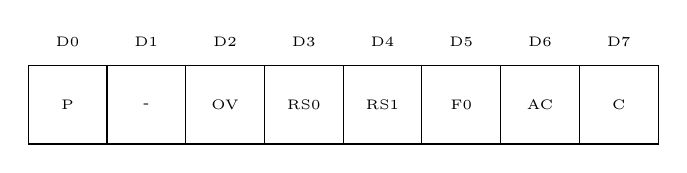
\begin{tikzpicture}
    \foreach \x/\label/\bit in {0/P/D0, 1/-/D1, 2/OV/D2, 3/RS0/D3, 4/RS1/D4, 5/F0/D5, 6/AC/D6, 7/C/D7} {
        \draw (\x,0) rectangle (\x+1,1);
        \node at (\x+0.5, 0.5) {\tiny \label};
        \node at (\x+0.5, 1.3) {\tiny \bit};
    }
\end{tikzpicture}
\end{center}

\textbf{Flag Functions:}
\begin{itemize}
    \item \textbf{C (Carry - D7)}: Set when carry/borrow occurs in arithmetic
    \item \textbf{AC (Auxiliary Carry - D6)}: Set when carry from D3 to D4 (BCD arithmetic)
    \item \textbf{F0 (D5)}: User defined flag
    \item \textbf{RS1, RS0 (D4, D3)}: Register Bank Select (00=Bank0, 01=Bank1, 10=Bank2, 11=Bank3)
    \item \textbf{OV (Overflow - D2)}: Set when signed arithmetic overflow occurs
    \item \textbf{P (Parity - D0)}: Set to 1 if Accumulator has odd number of 1s (Even Parity needed)
\end{itemize}
\end{solutionbox}
\begin{mnemonicbox}
``Carry Auxiliary Overflow Parity Register'' (CAOPR)
\end{mnemonicbox}

\questionmarks{5}{b}{4}
\textbf{Draw and explain diagram Interfacing 7 segment with microcontroller.}

\begin{solutionbox}
\textbf{Answer}:

\textbf{7-Segment Interface (Common Cathode):}

\begin{center}
\begin{tikzpicture}[node distance=3cm, auto]
    \node [gtu block] (8051) {8051\\(Port 1)};
    \node [gtu block, right of=8051, node distance=4cm] (driver) {Driver\\(ULN2003)};
    \node [gtu block, right of=driver, node distance=4cm] (disp) {7-Segment\\Display\\(Common Cathode)};
    
    \draw [->, thick] (8051) -- (driver) node[midway, above] {P1.0-P1.7};
    \draw [->, thick] (driver) -- (disp) node[midway, above] {a-g, dp};
    
    \draw [->] (disp.south) -- ++(0,-1) node[below] {GND};
    \draw [->] (driver.north) -- ++(0,1) node[above] {+5V};
\end{tikzpicture}
\end{center}

\textbf{Components:}
\begin{itemize}
    \item \textbf{ULN2003/Resistors}: Used as current driver/limiter because 8051 ports generally cannot drive LED segments directly (or use logic low to drive Common Anode).
    \item \textbf{Display}: Common Cathode type requires Logic 1 (High) to turn on segment (via driver).
\end{itemize}
\end{solutionbox}
\begin{mnemonicbox}
``Port Driver Display Ground'' (PDDG)
\end{mnemonicbox}

\questionmarks{5}{c}{7}
\textbf{Interface 8 LEDs with microcontroller and write a program to turn on and off.}

\begin{solutionbox}
\textbf{Answer}:

\textbf{LED Interface Circuit:}

\begin{center}
\begin{tikzpicture}[auto]
    \node [gtu block] (8051) {8051 Microcontroller};
    
    \foreach \i in {0,1,2,3,4,5,6,7} {
        \draw [->] (8051.east) ++(0, 1.75 - \i*0.5) coordinate (p\i) -- ++(1,0) node[right, draw, circle, scale=0.5] (led\i) {LED} -- ++(0.5,0) node[right] {+5V};
        \node [left] at (p\i) {P1.\i};
        \node [above] at ($(led\i)+(-0.3,0)$) {\tiny $R$};
    }
\end{tikzpicture}
\end{center}
\textit{Note: Diagram shows Common Anode configuration (Active Low) for simple driving.}

\textbf{Assembly Program:}
\begin{lstlisting}[language={[x86masm]Assembler}]
ORG 0000H           ; Start address
MAIN:
    MOV P1,#00H     ; Turn ON all LEDs (Logic 0 for Active Low)
                    ; If Active High: MOV P1,#0FFH
    ACALL DELAY     ; Wait
    MOV P1,#0FFH    ; Turn OFF all LEDs (Logic 1)
                    ; If Active High: MOV P1,#00H
    ACALL DELAY     ; Wait
    SJMP MAIN       ; Repeat continuously

DELAY:
    MOV R2,#250     ; Outer loop
D1: MOV R3,#250     ; Inner loop
D2: DJNZ R3,D2      ; Decrement inner
    DJNZ R2,D1      ; Decrement outer
    RET             ; Return
END
\end{lstlisting}
\end{solutionbox}
\begin{mnemonicbox}
``Light Emitting Display Interface'' (LEDI)
\end{mnemonicbox}

\orquestionmarks{5}{a}{3}
\textbf{List Applications of microcontroller in various fields.}

\begin{solutionbox}
\textbf{Answer}:

\begin{center}
\captionof{table}{Applications}
\begin{tabulary}{\linewidth}{|l|J|}
\hline
\textbf{Field} & \textbf{Applications} \\ \hline
\textbf{Home Appliances} & Washing machine, Microwave, AC, TV Remote \\ \hline
\textbf{Automotive} & Engine Control Unit (ECU), ABS, Airbags, Dashboard \\ \hline
\textbf{Industrial} & Process control, Robotics, Sensors, Automation \\ \hline
\textbf{Medical} & Pacemaker, Blood pressure monitor, Ventilators \\ \hline
\textbf{Communication} & Mobile phones, Modems, Routers \\ \hline
\textbf{Security} & Access control systems, Burglar alarms, CCTV \\ \hline
\textbf{Entertainment} & Gaming consoles, Music players, Toys \\ \hline
\end{tabulary}
\end{center}
\end{solutionbox}
\begin{mnemonicbox}
``Home Auto Industrial Medical Communication Security Entertainment'' (HAIMCSE)
\end{mnemonicbox}

\orquestionmarks{5}{b}{4}
\textbf{Draw and explain diagram interfacing of DC motor with 8051.}

\begin{solutionbox}
\textbf{Answer}:

\textbf{DC Motor Interface (using L293D):}

\begin{center}
\begin{tikzpicture}[node distance=3cm, auto]
    \node [gtu block] (8051) {8051};
    \node [gtu block, right of=8051, node distance=4cm] (driver) {L293D\\Driver};
    \node [gtu block, right of=driver, node distance=4cm] (motor) {DC\\Motor};
    
    \draw [->, thick] (8051) -- (driver) node[midway, above] {P1.1, P1.2};
    \draw [->, thick] (driver) -- (motor) node[midway, above] {Out1, Out2};
    
    \draw [->] (driver.north) -- ++(0,1) node[above] {+12V (Motor Supply)};
    \draw [->] (driver.south) -- ++(0,-1) node[below] {GND};
\end{tikzpicture}
\end{center}

\textbf{Operation using H-Bridge (L293D):}
\begin{itemize}
    \item \textbf{Forward}: P1.1 = 1, P1.2 = 0
    \item \textbf{Reverse}: P1.1 = 0, P1.2 = 1
    \item \textbf{Stop}: P1.1 = 0, P1.2 = 0 (or 1, 1)
\end{itemize}
\end{solutionbox}
\begin{mnemonicbox}
``Driver Control Motor Direction'' (DCMD)
\end{mnemonicbox}

\orquestionmarks{5}{c}{7}
\textbf{Interface LCD with microcontroller and write a program to display "Microprocessor and Microcontroller".}

\begin{solutionbox}
\textbf{Answer}:

\textbf{LCD Interface (16x2):}

\begin{center}
\begin{tikzpicture}[node distance=4cm, auto]
    \node [gtu block] (8051) {8051};
    \node [gtu block, right of=8051, minimum height=3cm] (lcd) {16x2 LCD};
    
    \draw [->, thick] (8051.20) -- (lcd.160) node[midway, above] {Data Bus (P1.0-P1.7)};
    \draw [->, thick] (8051.-20) -- (lcd.-160) node[midway, below] {Control (RS, RW, E)};
    
    \node [right] at (8051.east) {P2.0, P2.1, GND};
\end{tikzpicture}
\end{center}

\textbf{Assembly Program:}
\begin{lstlisting}[language={[x86masm]Assembler}]
ORG 0000H
    ACALL LCD_INIT      ; Initialize LCD
    MOV DPTR,#MSG       ; Point to message
DISP_LOOP:
    CLR A
    MOVC A,@A+DPTR      ; Get character
    JZ STOP             ; If 0, stop
    ACALL SEND_DATA     ; Display char
    INC DPTR            ; Next char
    SJMP DISP_LOOP      ; Repeat
STOP: SJMP $

LCD_INIT:
    MOV A,#38H          ; 2 lines, 5x7 matrix
    ACALL SEND_CMD
    MOV A,#0FH          ; Display ON, Cursor ON
    ACALL SEND_CMD
    MOV A,#01H          ; Clear Display
    ACALL SEND_CMD
    RET
    
SEND_CMD:
    MOV P1,A            ; Send command to Data Port
    CLR P2.0            ; RS=0 for Command
    CLR P2.1            ; RW=0 for Write
    SETB P2.2           ; E=1
    CLR P2.2            ; E=0 (Latch)
    ACALL DELAY
    RET

SEND_DATA:
    MOV P1,A            ; Send data to Data Port
    SETB P2.0           ; RS=1 for Data
    CLR P2.1            ; RW=0 for Write
    SETB P2.2           ; E=1
    CLR P2.2            ; E=0 (Latch)
    ACALL DELAY
    RET

DELAY: MOV R3,#50       ; Simple delay
       DJNZ R3,$ 
       RET

MSG: DB "Microprocessor and Microcontroller",0h
END
\end{lstlisting}
\end{solutionbox}
\begin{mnemonicbox}
``Init Send Data Display Message'' (ISDDM)
\end{mnemonicbox}

\end{document}
